\chapter{纠删码的高可靠预先数据修复算法研究}







\section{引言}

分布式存储系统通过对数据进行冗余来保证数据的可靠性和可用性,基于纠删码的冗余技术能减少存储空间。
在存储集群中利用多个节点来提供足够的数据冗余以降低数据丢失的可能性。
多备份冗余是创建了至少三份数据副本,但是在数据存储急剧增长的情况下,
备份冗余会引发大量存储开销,早期的分布式集群一般采用这种方式.
纠删码则是通过编解码矩阵的计算创建了远小于多备份技术的冗余数据,
同时提供同级别的容错性\cite{weatherspoon2002erasure}。如今的大规模存储群越来越多地采用纠删码\cite{ford2010availability,huang2012erasure,muralidhar2014f4,ovsiannikov2013quantcast},
以取得存储空间和可靠性的均衡。

纠删码面临的最基本问题就是过量的修复开销:
修复流量随着存储冗余度的降低而增加\cite{dimakis2010network}。因此,前人对改善纠删码的修复性能进行了广泛的研究,
使修复过程中的修复流量或I/O最小化\citep{dimakis2010network,huang2012erasure,sathiamoorthy2013xoring},
或设计适用于所有实践中的纠删码包括RS码的提高修复效率的技术\citep{bhagwan2004total,li2017repair,li2019openec,mitra2016partial,shen2016reconsidering,silberstein2014lazy}。
目前,大部分的传统修复方法都是被动修复,只有在检测到节点故障后才会触发修复操作。
如果可以提前预测即将发生的故障,就可以在任何实际故障发生之前主动修复任何即将发生的节点故障,以提高系统可靠性。

随着机器学习技术的不断发展,很多研究也将其与磁盘预测技术结合在一起进而提高预测精准度。
在某些情况下,预测精度甚至可以达到至少95\%\cite{botezatu2016predicting,li2014hard,mahdisoltani2017proactive,zhu2013proactive},
并且误报率非常小。故\citet{shen2019fast}定义了STF节点为根据预测技术得到的精确的即将故障的节点,在这前提下
通过耦合两种修复方法——迁移和重建提出了FastPR算法,准确定位STF节点并加速修复操作。然而在修复调度上,FastPR在带宽快速变化的网络环境中,尤其是在
带宽不对等的环境下修复性能会受到限制。

本文在FastPR对于STF节点修复任务的前提下, 进一步将其扩展到网络环境快速变化的情形中。利用空闲节点加速数据的传输并感知当前网络环境的变化。

\section{预先修复问题建模}
本文通过结合迁移与重建来设计实现预先修复的机制,用以修复STF(Soon To Fail)\cite{shen2019fast}节点。
这两种修复方式各有其优缺点,迁移是直接从一个STF节点上读取存储的编码与数据块,将其重新传输到一个或多个正常的节点中,
与常规读取相比,它并不会引发额外的带宽消耗。然而,迁移的性能却受到STF节点可用带宽的限制,另一方面,
重建修复遵循着传统的反应式修复,亦即只有当节点数据不可访问时才会触发修复机制,
通过从可用节点中检索多个条带来重建STF节点的数据条带。由于这些数据与编码条带通常分布在存储集群中,
可以利用存储集群的可用带宽资源,让所有可用节点以并行的方式参与STF节点的多个条带的修复,但是会引发额外的带宽消耗。

\subsection{问题描述}

以$RS(5,3)$为例,其中$n=5$和$k=3$,设$N_i$为第$i$个可用节点, 
$S_i$是要修复的STF节点的第$i$个块的条带。假设现在得到了一个STF节点的$c_m$和$c_r$的集合,
其中$c_m$为迁移的块的个数,$c_r$为重建的块的个数。如图~\ref{fig:3.2}所示的存储集群,总共有$M=7$个节点,其中$M-1=6$个可用节点,
$N_1,N_2,\cdots,N_6$,而STF节点的块对应于条带$S_1,S_2,S_3$。


\citet{shen2019fast}提出,对于这样的通常情况需要解决两个基本问题,
其一是在给定的通过重建修复的STF节点的$c_r$块中,
需要确定从$k-c_r$个可用节点中检索出$k-c_r$个块,将$k-c_r$的检索选择表述为一个二分图最大匹配问题。
其二是需要确定存储$c_m+c_r$个修复后的块。一般而言,将修复的块存储在$c_m+c_r$个现有的可用节点中,
这样就可以保持节点的容错性,即任何$n-k$个节点的故障都是可以容忍的,再次将选择$c_m+c_r$个可用节点表述为二分图最大匹配问题。

然而在实际分布式网络修复中,不仅仅只关注需要用到哪些块进行修复与存储,
其中并行的性能还受到节点之间的快速变化的带宽和文件访问频次的影响。
首先按照在一个存储集群中对于不同种类的数据访问频次的不同,
包含相应文件的节点宕机造成的损失要远高于存放那些不常用的数据的节点宕机所造成的损失,
这种情况在预先修复中就需要纳入考虑,提高对热数据的修复顺序的权重可以极高地增加存储集群的可靠性与持久性;
其次,对于一个STF节点而言,存储着来自不同数据的数据块与校验块,如何确定当前所需要的块的修复方法也是至关重要的。
在快速变化的网络环境中,可用节点并行地处理修复任务与迁移任务,不同节点的带宽瓶颈不同,
如果在修复过程中随机选择迁移或者重建方法,势必会造成整个网络修复性能得不到充分利用,
或者某个节点超出负荷的运行而剩下的节点却处于空闲状态,
需要设计一个算法充分利用整个网络的带宽进行重建与迁移,其中至关重要的就是对于一个STF节点确认其重建集$c_m$与迁移集$c_r$。 

问题转化为计算出$c_m$和$c_r$的集合,亦即确定重建集和迁移集的具体块。
有如下具体问题,若一个STF节点拥有$m+r$个数据块,每个块对应的文件有着相应的访问热度$T_i(1\leqslant n \leqslant m+r)$,
且在可用节点中,$w_{nj}$表示$n$节点到$j$节点实时带宽速度,每个节点拥有$t$个数据块,分别为$[N_s,\cdots,N_k,\cdots,N_t](s<k<t)$,
以及每个节点是否处于参与修复任务状态位$State_n$,取值为$\{T,F\}$,现在需要确定当STF节点产生时,
其中的数据块通过耦合重建和修复达到修复时间最短的方案。

\subsection{模型假设}
修复技术的主要目标就是减少修复时间,并且最大化地利用实时带宽。为此我们做出如下假设:

\begin{enumerate}
	\item 存储集群每次最多只有一个STF节点,这是基于单节点修复是最主要的修复事件,且占据修复事件总数的98\%\cite{rashmi2013solution}。
	\item 随着系统运行,配备的预测算法预测出的STF节点的成功率是100\%。
	\item STF节点中的分块在修复过程中仍然可以访问,直到STF节点实际发生故障。
	\item 在多次修复后,块分布可能会变得不平衡,假设集群拥有自动再平衡的能力。
\end{enumerate}

\subsection{理论修复时间}
\label{subsection3.1}

设$M$为存储系统中的节点总数,$U$为STF节点需要被修复的块的总量。设$x$是被迁移修复的块的数量,则$U-x$是重建修复的块的数量。对于迁移修复,
$t_m$为将一个块从STF节点迁移到另一个正常节点的时间,因此总的迁移时间为$x \cdot t_m $。对于重建修复,
令$t_r$为修复STF节点的一个块的时间。在$RS(n,k)$的设置下,$k$个正常节点需要搜索$k$个块来重建STF节点的
每个块,若$M-1$个正常节点数远大于$k$,则可以同时重建STF节点的多个块。假设重建修复可分为多轮,那么在每一轮
中,可以找到$G\leqslant \frac{M-1}{k}$个不重叠的组,这些组中的$k$个节点属于不同的条带,并可以从这些
组并行地搜索出$k$个块。因此,可以在$t_r$时间内通过重建修复STF节点的$G$个块,重建消耗的总时间为$\frac{U-x}{G} \leqslant t_r$。

令$T(x)$为预先修复的总时间,又重建和迁移是并行执行的,则:
\begin{equation}
	\label{eq:3-1}
	T(x)=\max \left(x \cdot t_{m}, \frac{U-x}{G} \cdot t_{r}\right)
\end{equation}

当$x \cdot t_m = \frac{U-x}{G} \cdot t_r$时,$T(x)$最小,也就是$x = \frac{U \cdot t_{r}}{G \cdot t_{m}+t_{r}}$。因此,最小的
预先修复时间$T_P$为:
\begin{equation}
	\label{eq:3-2}
	T_{P}=\frac{U \cdot t_{r} \cdot t_{m}}{G \cdot t_{m}+t_{r}}
\end{equation}

对于反应式修复只会进行重建,则总的修复时间为$T_R$则为式~\ref{eq:3-1}中,当$x=0$时的$T(0)$:
\begin{equation}
	\label{eq:3-3}
	T_{R}=\frac{U \cdot t_{r}}{G}
\end{equation}

\subsection{迁移与重建时间建模}
本文将修复过程分解为三个部分,并按照顺序方式进行。(1)读取,从本地存储中读取数据块;(2)传输,通过网络进行数据传输;(3)写入,将修复后的数据写入
正常节点。设$b_d$和$b_n$分别为磁盘和网络带宽,$c$是块大小。首先对于迁移任务,对于每个块的读取时间为$\frac{c}{b_d}$,传输时间为$\frac{c}{b_n}$,
写入时间为$\frac{c}{b_d}$,则$t_m$有:
\begin{equation}
	\label{eq:3-4}
    t_{m}=\frac{2c}{b_{d}}+\frac{c}{b_{n}}
\end{equation}

对于重建任务,$k$个正常节点可以并行地读取同一条带的块,故对每一个待读取块的读取时间为$\frac{c}{b_d}$。因为接收$k$个块的节点一个时间步只能接收一个块,
故所有$k$个块的传输时间为$k \cdot \frac{c}{b_n}$,正常节点接收了所有$k$个块后进行矩阵计算(这里忽略计算时间)得出一个数据块写入正常节点,故写入
时间为$\frac{c}{b_d}$,因此$t_r$有:
\begin{equation}
	\label{eq:3-5}
    t_{r}=\frac{2c}{b_{d}}+\frac{k \cdot c}{b_{n}}
\end{equation}

设$M=100$,$U=1,000$,块大小$c=64MB$,$b_d=100MB/s$,且$b_n=1Gb/s$。考虑$RS(9,6)$,$RS(14,10)$,$RS(16,12)$三种分布式存储系统中的
常见RS码配置。如图~\ref{fig:3.1}所示,当节点数较少、$k$较大、$b_d$较大、$b_n$较小时,分别对应了~\ref{fig:3-1},~\ref{fig:3-2},~\ref{fig:3-3},~\ref{fig:3-4}四张子图,
预先修复的性能要反应式修复更加高效。
总的来说,预先修复在所有情况下都减少了反应式修复的修复时间,例如,在$RS(16, 12)$中减少了33.1\%(图~\ref{fig:3-2})。


\begin{figure}[htbp]
	\centering
	\begin{subfigure}[t]{0.4\textwidth}
		\centering
		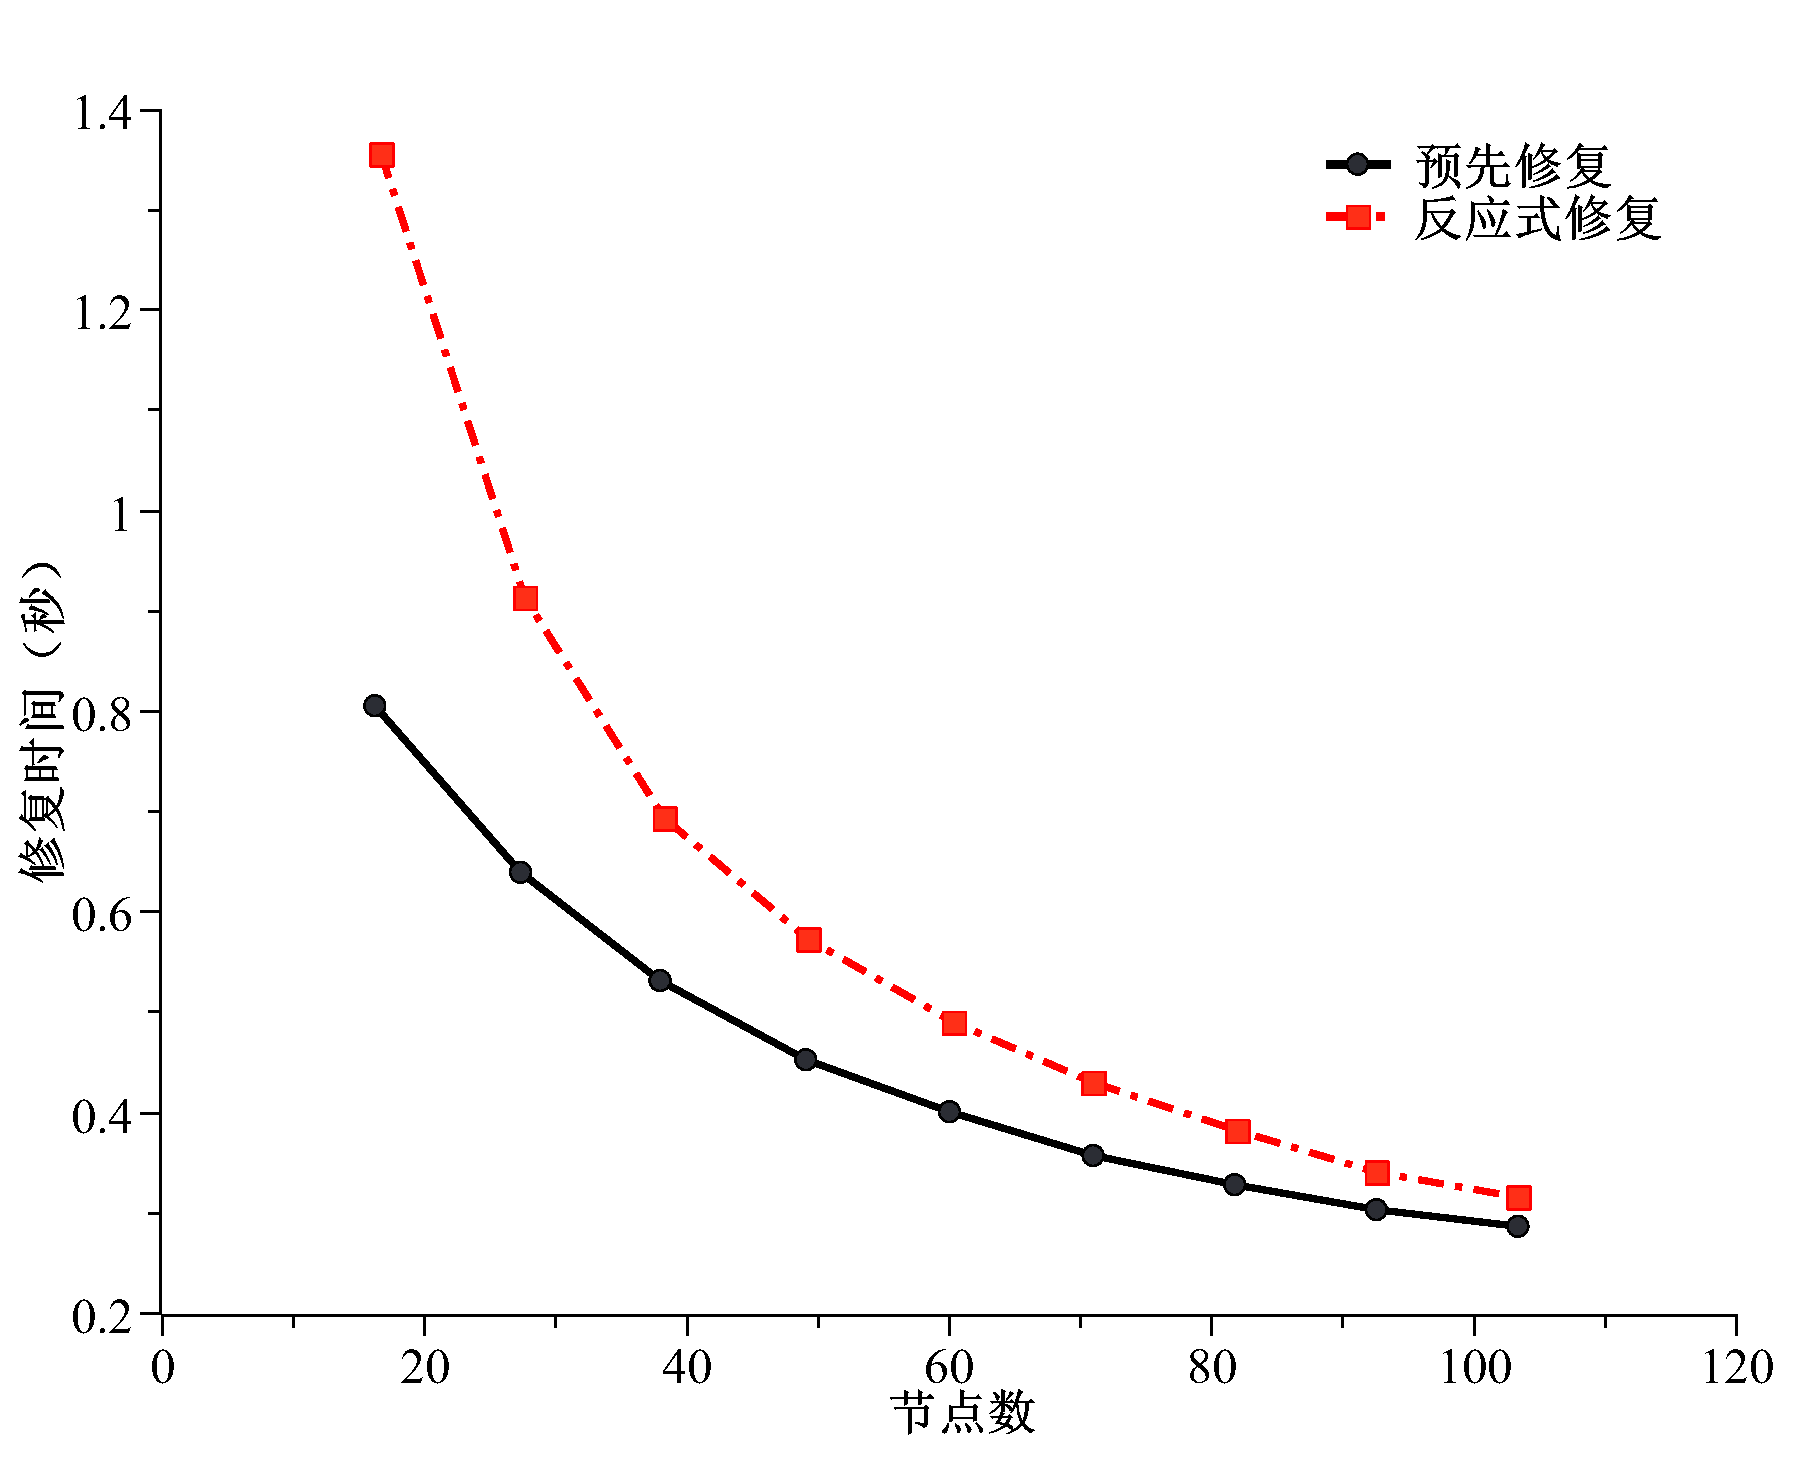
\includegraphics[width=1.1\linewidth]{figures/3-1.pdf}
		\caption{总节点数$M$值理论结果}
		\label{fig:3-1}
	\end{subfigure}
	\begin{subfigure}[t]{0.4\textwidth}
		\centering
		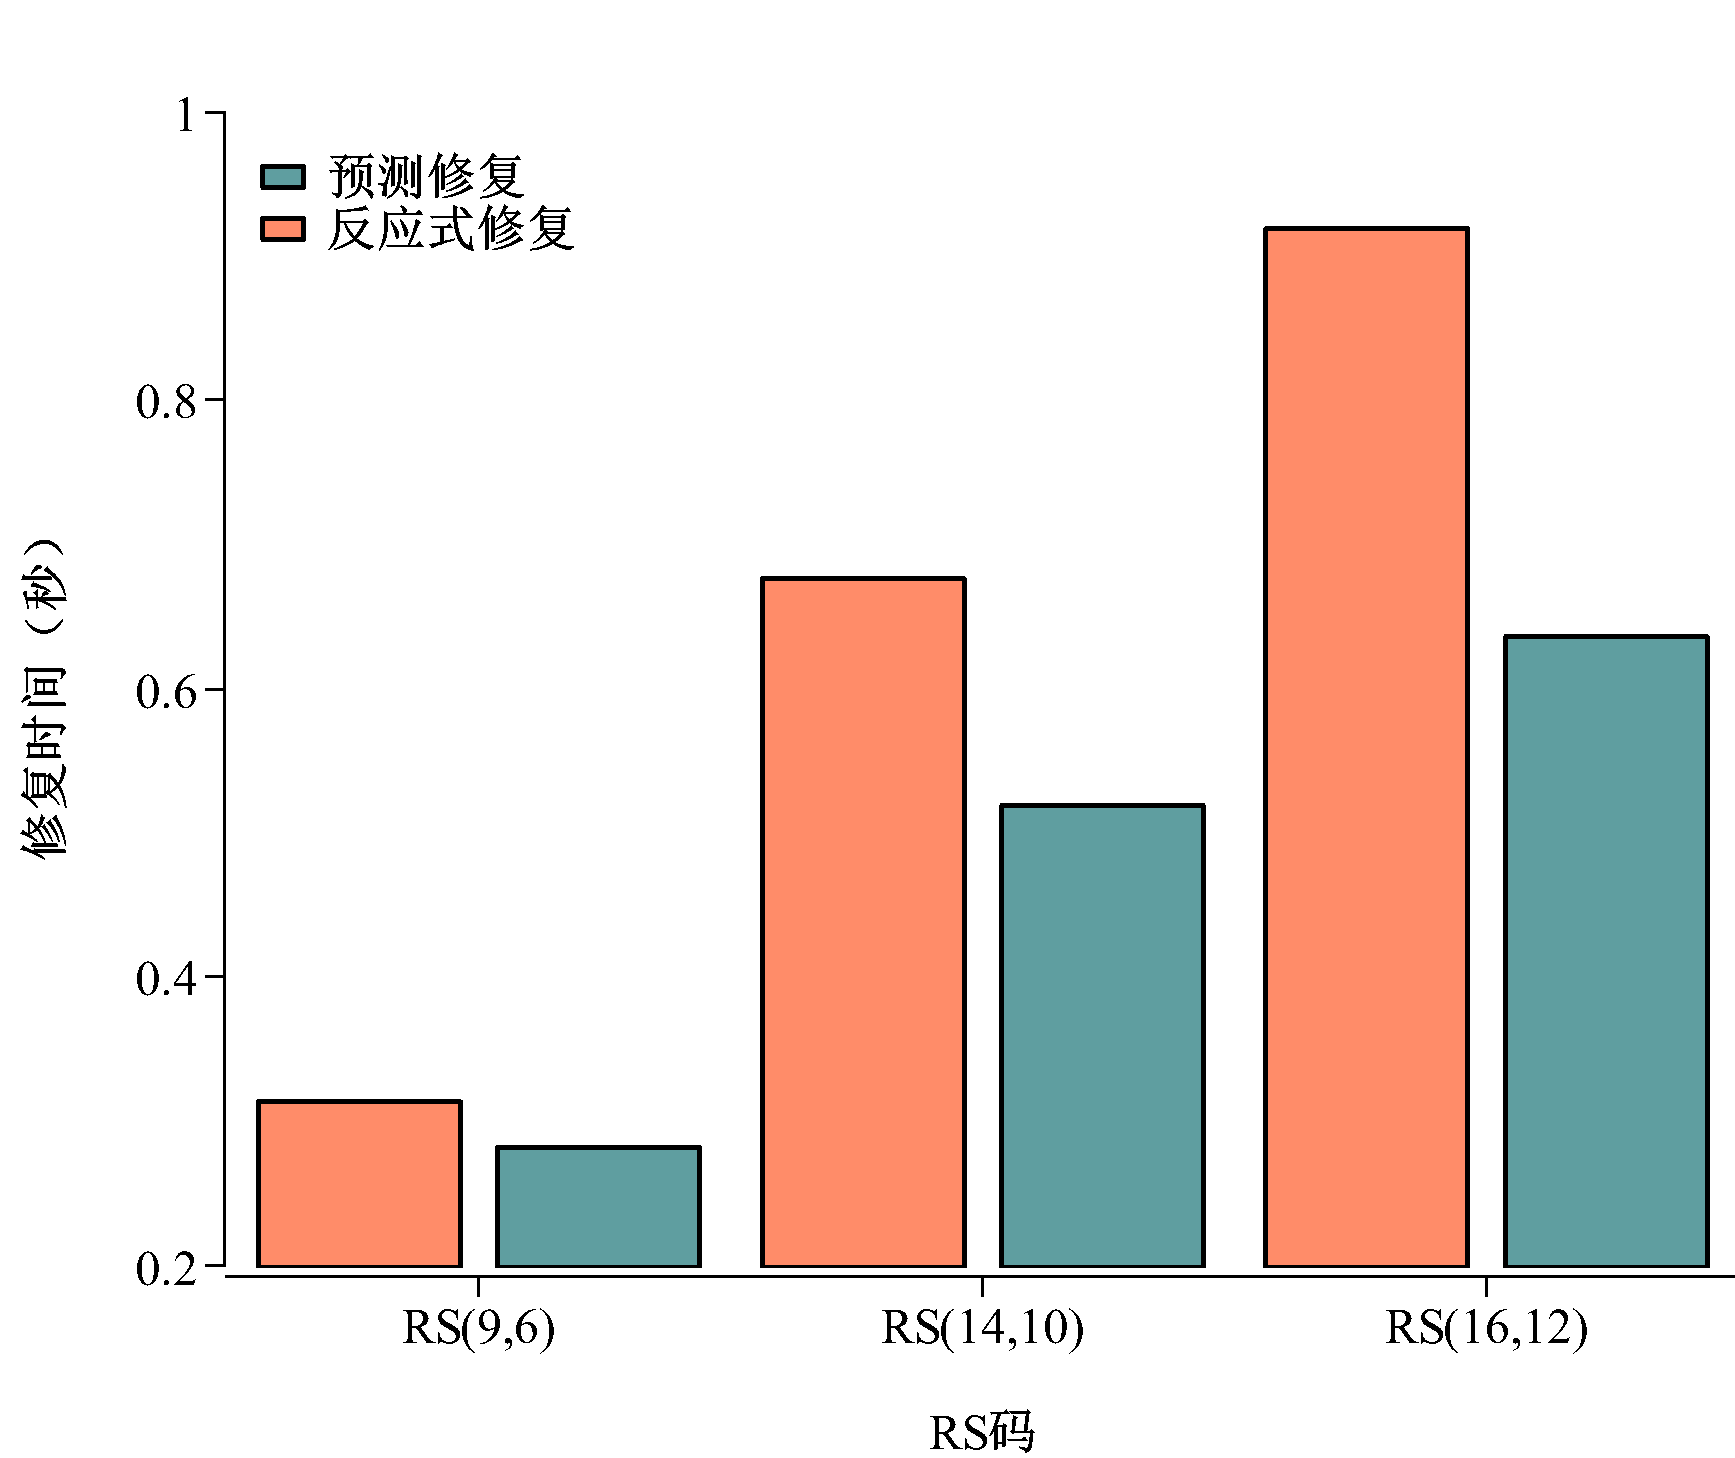
\includegraphics[width=1.2\linewidth]{figures/3-2.pdf}
		\caption{$RS(n,k)$配置理论结果}
		\label{fig:3-2}
	\end{subfigure}
	\begin{subfigure}[t]{0.4\textwidth}
		\centering
		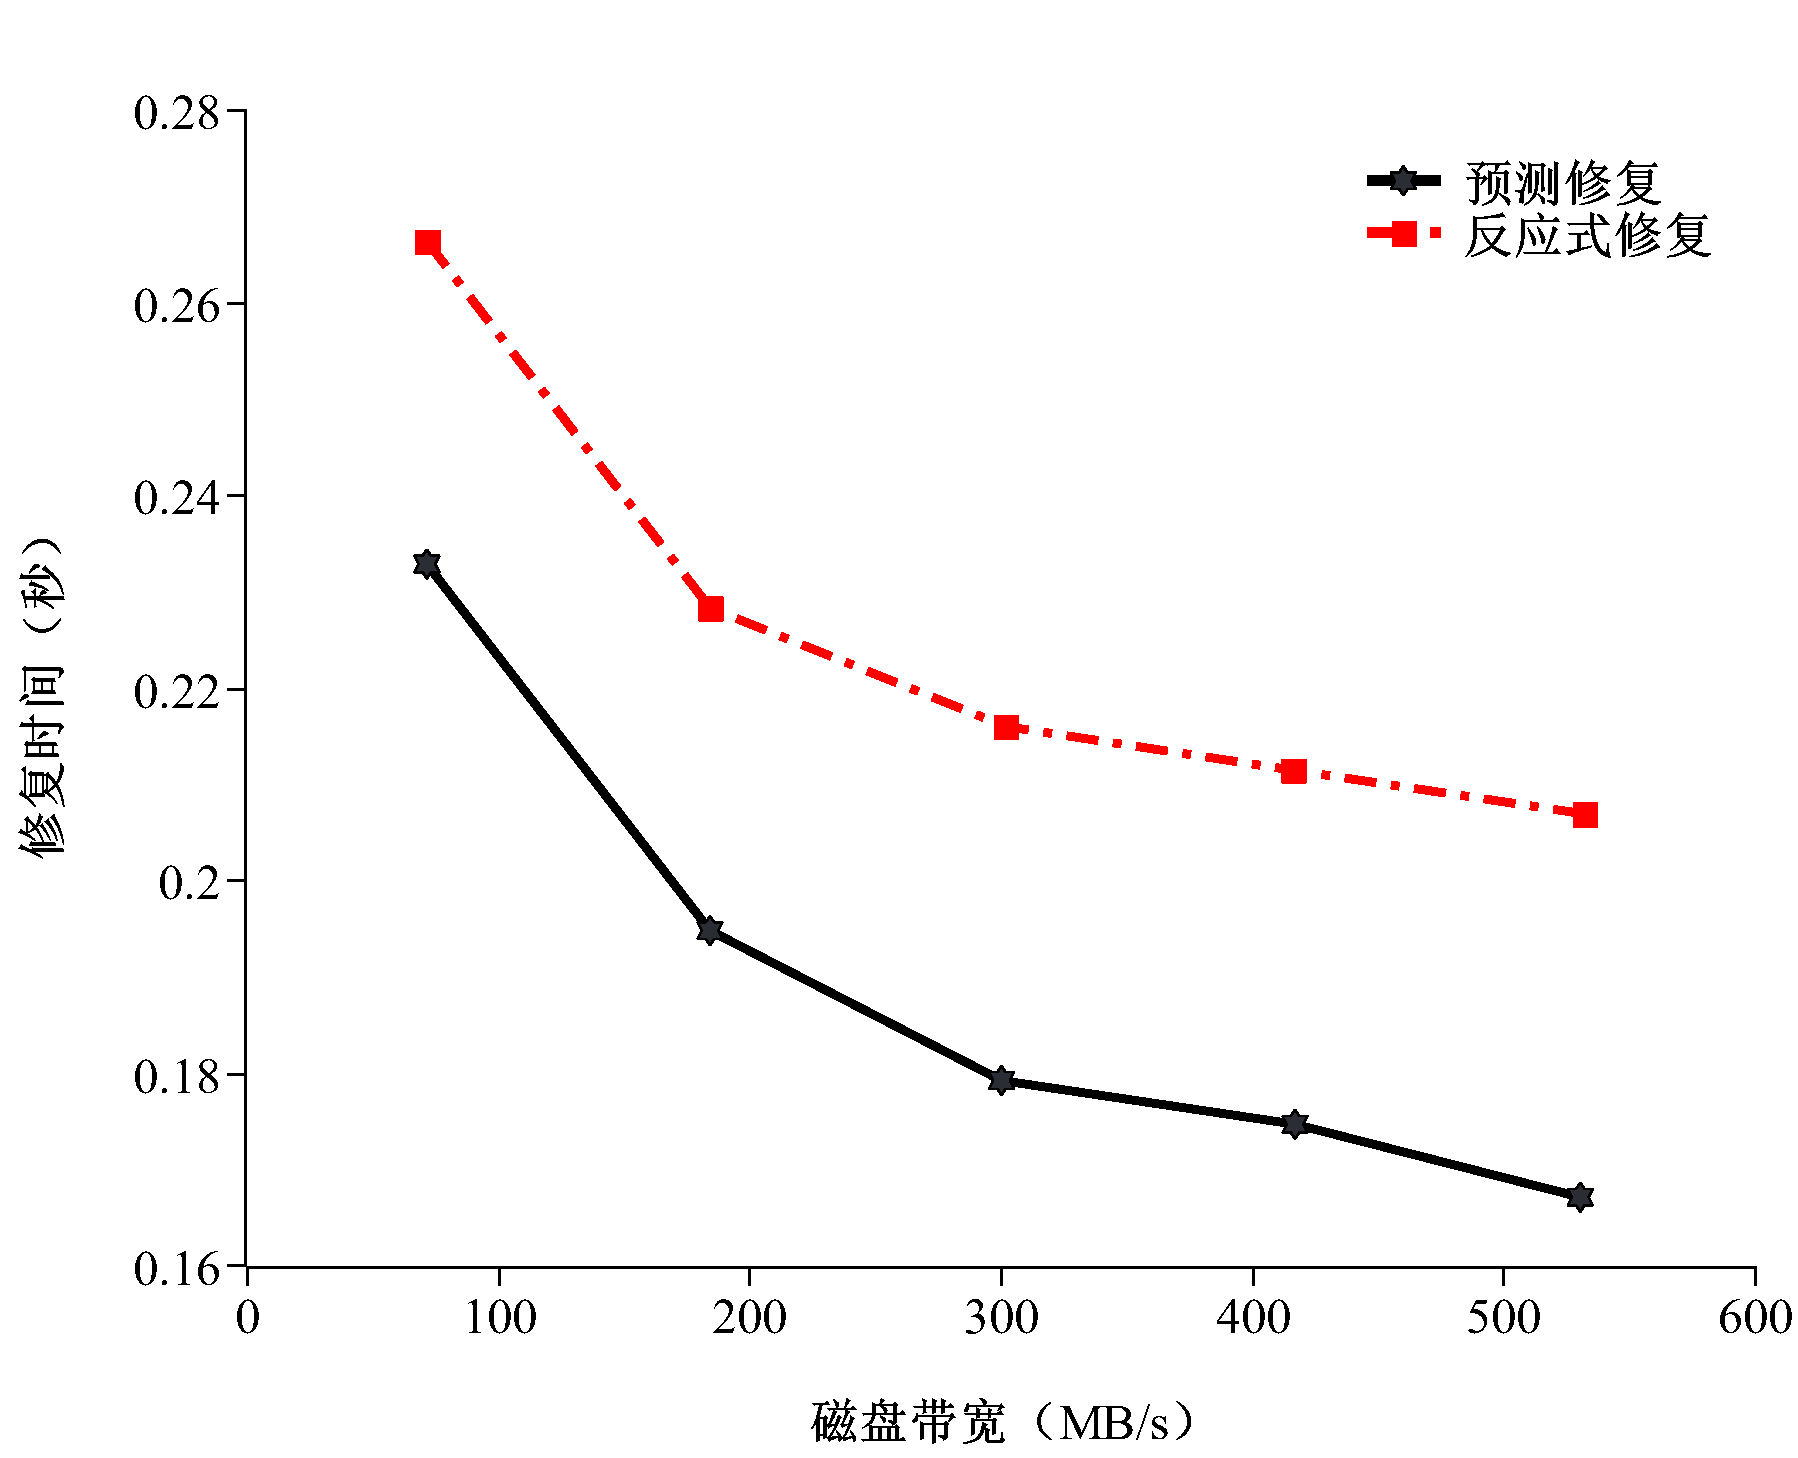
\includegraphics[width=1.1\linewidth]{figures/3-3.pdf}
		\caption{磁盘带宽$b_d$理论结果}
		\label{fig:3-3}
	\end{subfigure}
	\begin{subfigure}[t]{0.4\textwidth}
		\centering
		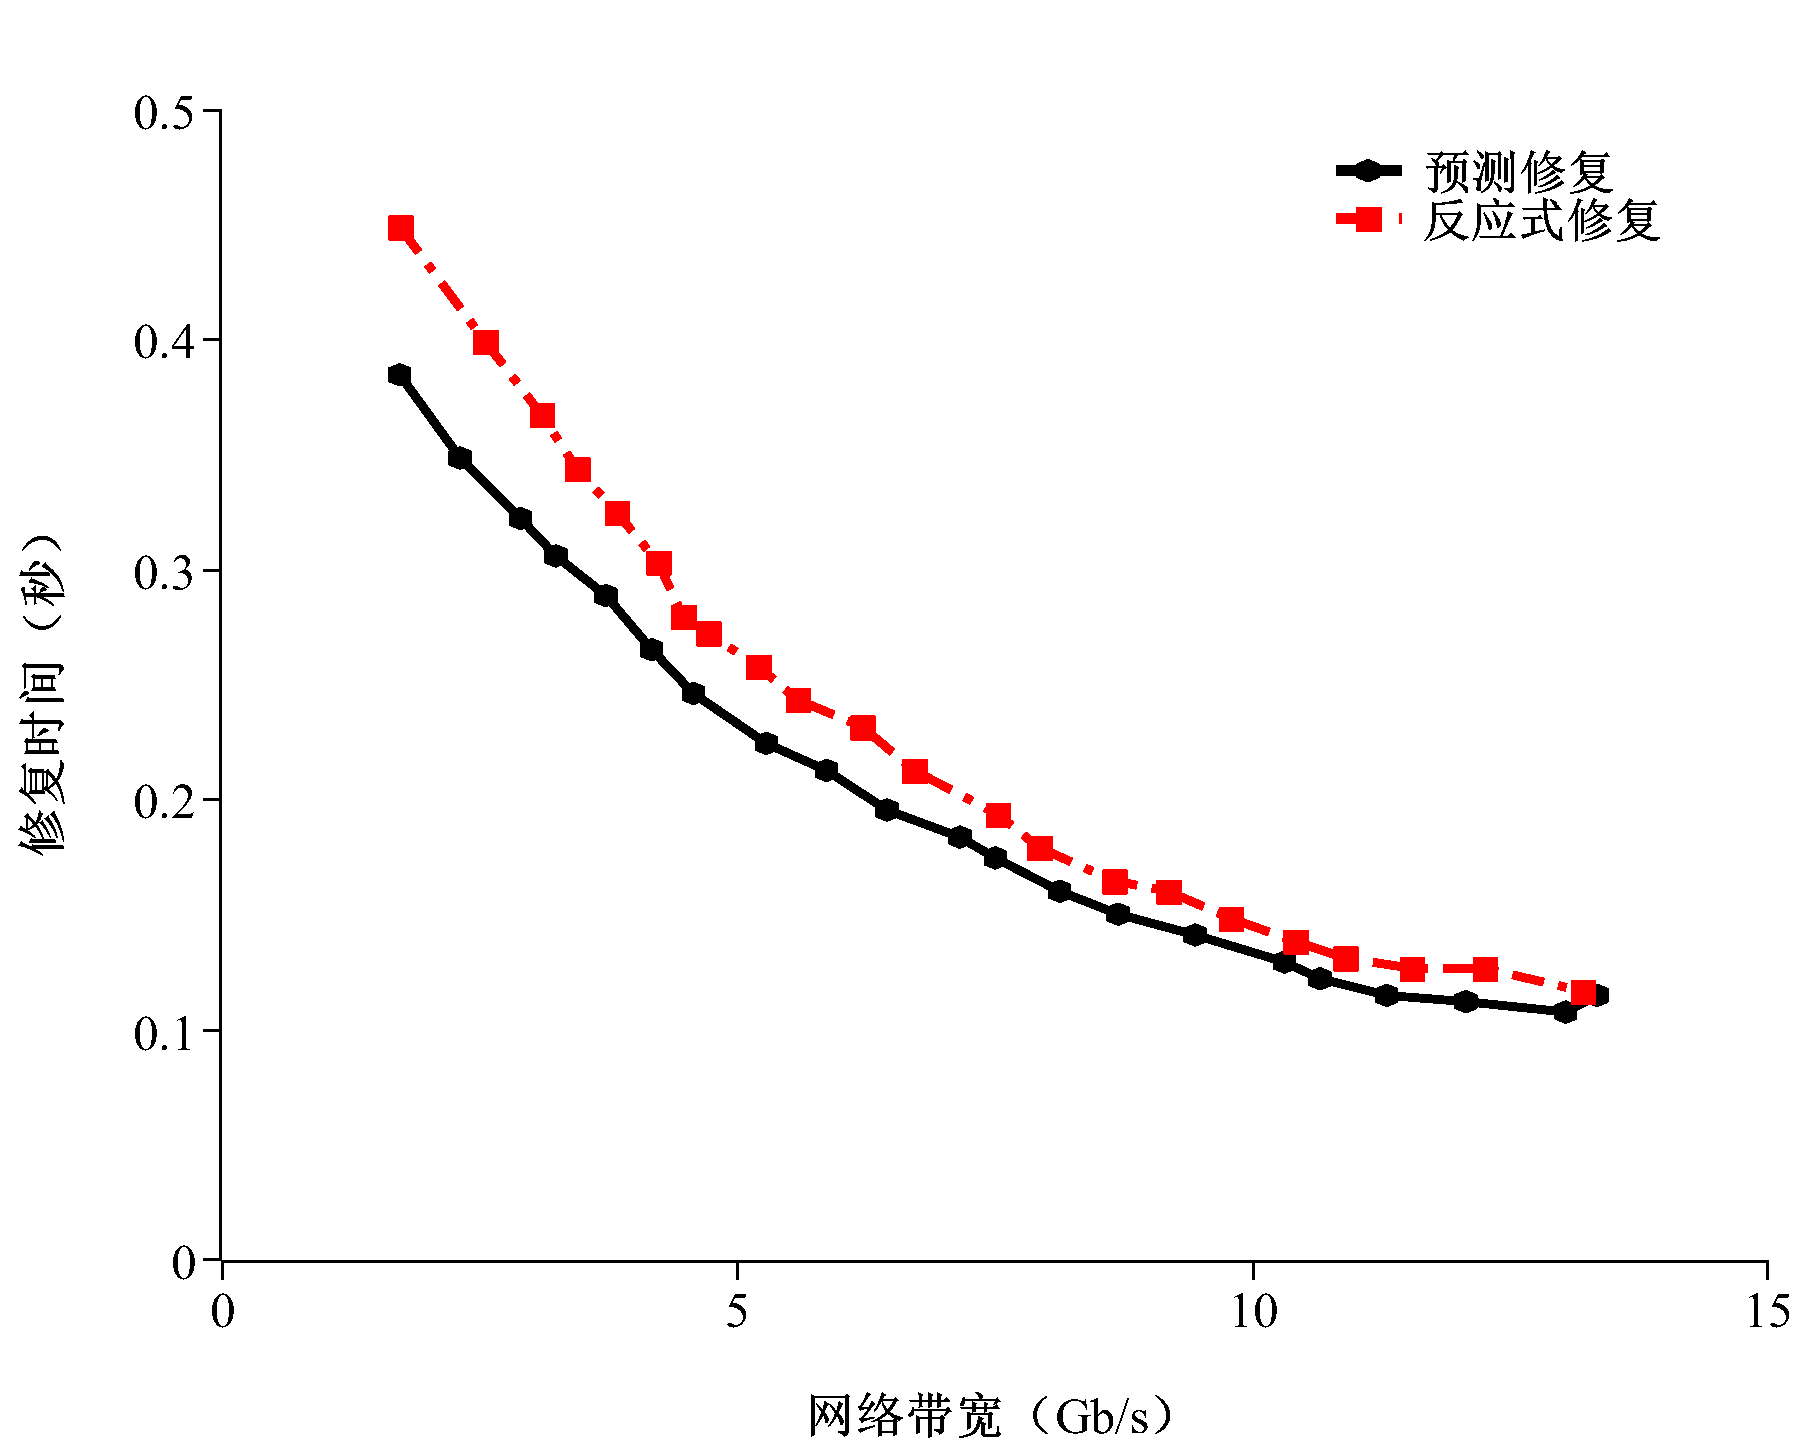
\includegraphics[width=1.1\linewidth]{figures/3-4.pdf}
		\caption{网络带宽$b_n$理论结果}
		\label{fig:3-4}
	\end{subfigure}
	\caption{预测修复与反应式修复建模对比}
	\label{fig:3.1}
\end{figure}


\section{预先修复集合划分算法}
在FastPR\cite{shen2019fast}中,算法的目标是最大限度地在每轮修复中增加STF节点的块的数量。假设STF节点中的所有块都要
通过重建方法进行修复,即从$k$个正常节点中获取$k$个块,这样中最多可以从$M-1$个正常节点每个节点获取一个块,这样就可以
在一个修复轮次中完成修复任务。
所以为了提高并行性,应该最大化重建集的块数量,如章节~\ref{subsection3.1}所说,最大为$\frac{M-1}{k}$。

本文针对重建集与迁移集问题,设计了划分迁移集与重建集算法SMSRS(Split Migration Set And Reconstruction Set)算法,如算法\ref{alg:3-1}所示。
该算法主要使用数据热度队列与最小堆技术,根据数据访问热度高低处理待修复的块的出队修复顺序,
利用最小堆不断优化当前出堆的网络带宽性能最优的可用节点进行迁移修复,然后通过贪心策略确定最佳的重建节点以及对应的重建块接收节点。

在获得迁移集$c_m$和重建集$c_r$中,需要先根据文件访问热度对相应文件的数据块进行排序送入队列$Q$(第1$\sim$2行),
按照热度从高到低的顺序从队列$Q$中弹出STF节点中待修复的块,
将其对应的节点编号按照与可用节点当前连接带宽的大小进行小堆化,
这样可以保证每次在堆顶取出当前与STF节点连接带宽速度最快的节点进行修复(第4$\sim$5行)。
在可用节点中找出当前不含有该STF节点待修复块的节点集$S_1$,并且不断从堆顶取出节点编号,
判断该节点是否处于执行修复任务状态以及是否包含于节点集$S_1$,若是则跳出,然后将不满足条件但弹出堆的数据再放回堆中,
并计算通过迁移块修复所耗费的时间$t_m$(第6$\sim$16行)。在可用节点中找出当前含有该STF节点待修复块的节点集$S_2$,并且定义带宽集$\textbf{D}$,
表示的是节点集$S_2$与可用节点集$\textbf{N}-S_2$中带宽各个节点传输的实时带宽值,在节点集$S_2$确定$r$个节点,
并在可用节点集中找出与这$r$个节点连接带宽值最大的节点$RNode$,
然后得出$r$个节点中与$RNode$连接最慢的节点除以块大小即得出对应的通过重建块修复所耗费的时间$t_r$(第17$\sim$30行)。
最后通过判断$t_r$和$t_m$的大小来确定重建集和迁移集,当队列$Q$为空时,则结束整个算法,返回相应的迁移集$c_m$和重建集$c_r$(第31行$\sim$39行)。
如图~\ref{fig:3.3}所示,展示了相应的流程。


\begin{figure}[htbp]
	\centering
	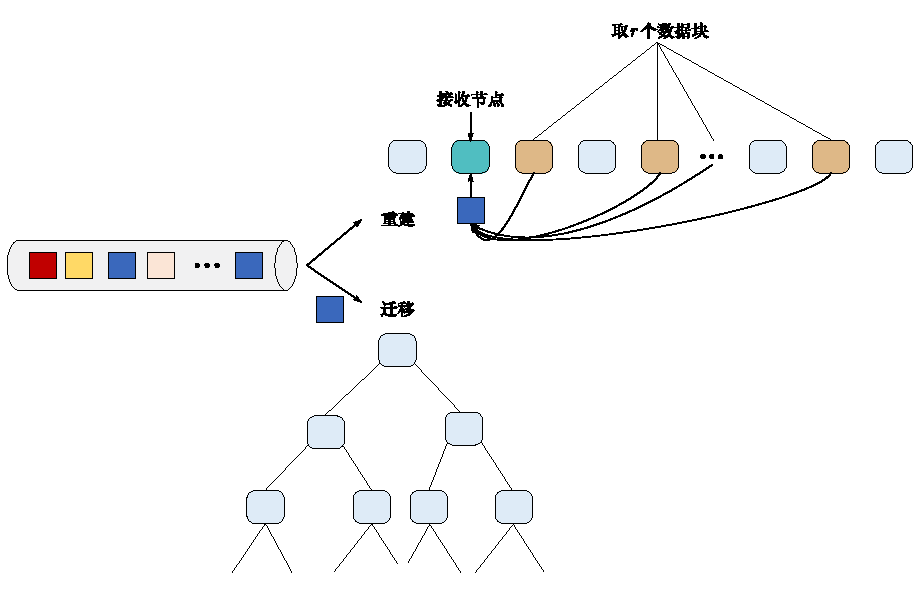
\includegraphics [scale=0.7]{figures/3.3.pdf}
	\caption{重建与迁移修复流程}
	\label{fig:3.3}
\end{figure}


\renewcommand{\algorithmicrequire}{\textbf{Input:}} % Use Input in the format of Algorithm
\renewcommand{\algorithmicensure}{\textbf{Output:}}


\begin{algorithm}[htpb]
	\begin{algorithmic}[1]
		\newlength{\commentindent}
		\setlength{\commentindent}{.3\textwidth}
		\setlength{\algorithmicindent}{1.5em}
		\renewcommand{\algorithmiccomment}[1]{\unskip\hfill\makebox[\commentindent][l]{$\rhd$~#1}\par}
		\LetLtxMacro{\oldalgorithmic}{\algorithmic}
		\renewcommand{\algorithmic}[1][0]{
			\oldalgorithmic[#1]
			\renewcommand{\ALC@com}[1]{
				\IFnum\pdfstrcmp{##1}{default}=0\ELSE\algorithmiccomment{##1}\fi}%
		}
		% \STATE \textbf{define:} $I,S,C \in \mathbb{R}^{n \times n \times B}$ \COMMENT{$B$ is \#sents in a batch}
		% \STATE \textbf{initialize:} $C_{i, i}  = 0, 0 \le i \le n$

		% \FOR [span width]{$w = 1$ \TO $n$}
		% \STATE \textbf{BatchIFy:} $0 \le i$; $j=i+w \le n$
		% \STATE $I_{i, j} = \log\left(\exp\left(C_{i, i}  +  C_{j, i+1}\right) ~ +\sum\limits_{i < r < j} \exp\left(I_{i, r} + S_{r, j}+ \mathrm{s}(i\rightarrow \{r,j\})\right)\right) + \mathrm{s}(i\rightarrow j)$
		% \STATE $S_{i, j} = \log \sum\limits_{i \le r < j} \exp\left(C_{i, r}  +  C_{j, r+1}\right) $ \\
		% \STATE $C_{i, j} = \log \sum\limits_{i < r \le j} \exp\left(I_{i, r}  +  C_{r, j}\right)  $ \\
		% \ENDFOR \COMMENT{refer to Fig.~\ref{fig:eisner-2o}}
		% \RETURN $C_{0, n} \equiv \log Z(\boldsymbol{x})$
		\REQUIRE
		ChunkSize, $m$, $r$, $\textbf{w}= \{ w_{i,j} \}$, $\textbf{N}= \{ N_{i} \}$, $\textbf{State}= \{ State_{i} \}$,$\textbf{T}= \{ T_{i} \}$;
		\ENSURE
		$c_m$, $c_r$;
		\STATE $c_m,c_r,TempSet = \emptyset$;
		\STATE Q $\gets$ SortedByAccessHeat($m+r$, $\textbf{T}$);
		\WHILE{true}
		\STATE STFNodeChunk = Q.pop();
		\STATE WHeap $\gets$ HeapIFy($j$, key=$w_{STFNodeChunk,j}$($ j \in$ $\textbf{N}$));
		\STATE $S_1$ = FindSTFNodeChunkNotIn(STFNodeChunk,$\textbf{N}$);
		\WHILE{true}
		\STATE  AvailableNode = WHeap.pop(); 
		\IF { $STATE_{AvailableNode} == T$ and AvailableNode $\in$ $S_1$ }
		\STATE break;
		\ELSE
		\STATE TempSet $\gets$ TempSet $\cup$ AvailableNode;
		\ENDIF
		\ENDWHILE
		\STATE WHeap.push(TempSet);
		\STATE $t_m$ = ChunkSize / $w_{STFNodeChunk,AvailableNode}$;
		\STATE $S_2$ = FindChunkIn(STFNodeChunk,$\textbf{N}$);

		\STATE $\textbf{D} = \emptyset $;
		\FOR{$n_1$ $\in$ $S_2$}
		\STATE $\textbf{DTemp} = \emptyset $;
		\FOR{$n_2$ $\in$ $\textbf{N} - S_2$}
		\STATE $\textbf{DTemp} \gets \textbf{DTemp} \cup w_{n_1,n_2}$;
		\ENDFOR
		\STATE $\textbf{D} \gets \textbf{D} \cup \textbf{DTemp} $;
		\ENDFOR
		\STATE $\textbf{TNode},RNode \gets$ FindMaximizedBandwidthTransferAndReceiveNode $(\textbf{D})$;
		\FOR{$n$ $\in$ $\textbf{TNode}$}
		\STATE Bdh = MIN($w_{n,RNode}$);
		\ENDFOR
		\STATE $t_r$ = ChunkSize / Bdh;
		\IF { $t_m < t_r$}
		\STATE $c_m \gets c_m \cup $ STFNodeChunk;
		\ELSE
		\STATE $c_r \gets c_r \cup $ STFNodeChunk;
		\ENDIF
		\IF { Length(Q) == 0}
		\STATE break;
		\ENDIF
		\ENDWHILE
		\STATE $\textbf{return} \quad c_m,c_r$
	\end{algorithmic}
	\caption{SMSRS算法}
	\label{alg:3-1}
\end{algorithm}





\section{预先修复调度算法}
常用的调度算法为单节点传输算法,亦即从源头节点直接传输数据到目标节点。但是这种方式往往会忽略通过高链路带宽传递数据带来的更快的修复速度的优势。
进而引出了多级传输的技术概念,亦即源节点数据在传递到源节点之前经过中继节点的转发,可以在更好地利用中间节点的高带宽优势的同时提高传输的并行性。
如PPR\cite{mitra2016partial},RP\cite{li2017repair},PPT\cite{bai2019fast}等技术都利用了这种技术特性提高了调度速度。

受\citet{zhou2022bandwidth}启发,本文提出了ISA(Improved SMFRepair Algorithm)算法来进行节点修复的调度。如图~\ref{fig:3.3}所示,
考虑$RS(5,3)$,修复一个失效的节点需要从$k$个$helper$节点钟获取$k$个数据块,其中$helper$节点由平均带宽进行确定。
对于$n$个节点${N_1,N_2,\cdots,N_n}$,$N_i$的平均带宽就是$Ave_BW_i=\frac{\sum_{j=1, j \neq i}^{n} \text { Bandwidth }{ }_{N i-N j}}{n-1}$。
例如,根据表~\ref{table:3-1}\cite{zhou2022bandwidth}图~\ref{fig:3.3}中的$D_2$的所在节点的平均带宽为
$(2+5+3+2)/4=3MB/s$。可以计算出所有$M-1$个节点的平均带宽,并选择平均带宽最大的$k$个节点作为$helper$节点。平均带宽
可以更直观地显示节点的传输数据的能力,平均带宽越大,那么低带宽的情况就会相对少见。

\begin{figure}[htbp]
	\centering
	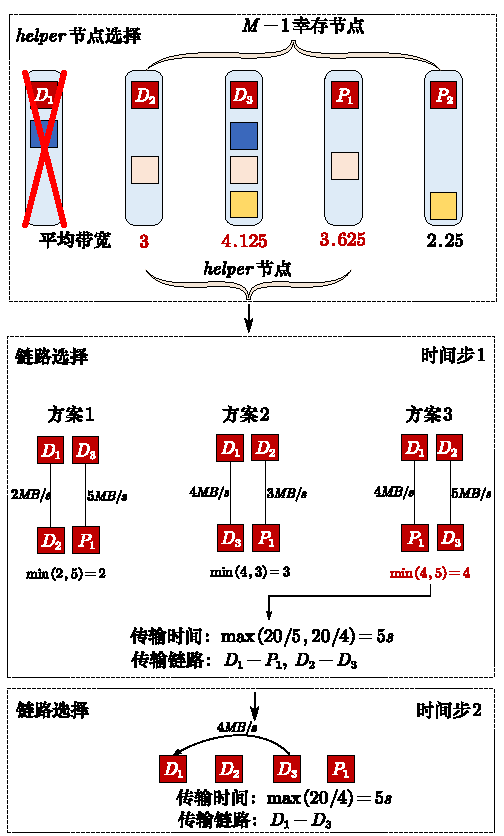
\includegraphics [scale=0.9]{figures/3.4.pdf}
	\caption{$helper$节点选择和链路选择过程图}
	\label{fig:3.4}
\end{figure}

\begin{table}[tb!]
	% \setlength{\tabcolsep}{2.9pt}
	\centering
	\caption{7个节点测量带宽(MB/s)}
	% \begin{tabularx}{\textwidth}{lccccccc}
        % \resizebox{\textwidth}{!}{
	\begin{tabular}{ccccccccc}
		\toprule
		\textsc{带宽}                       & \textsc{$D_1$}    & \textsc{$D_2$}    & \textsc{$D_3$}    & \textsc{$P_1$}   & \textsc{$P_2$}      & \textsc{$I_1$}   & \textsc{$I_2$}      \\[1pt]
		\midrule
		\\[-15pt]
		\textsc{$D_1$}                      & *              & 2              & 4           & 4       & 2       & 8      & 4         \\
		\textsc{$D_2$}                      & 2              & *              & 5           & 3       & 2       & 10      & 5        \\
		\textsc{$D_3$}                      & 4              & 5              & *           & 5       & 2.5     & 10      & 5        \\
		\textsc{$P_1$}                      & 4              & 3              & 5           & *       & 2.5     & 10      & 5        \\
		% \multicolumn{14}{c}{using raw text}                                                                                                                                                                                                                                                                                                                                                                                                                              \\[1pt]
		\textsc{$P_2$}                      & 2              & 2              & 2.5         & 2.5     & *       & 5      & 8         \\
		\textsc{$I_1$}                      & 8              & 10             & 10          & 10      & 5       & *      & 5         \\
		\textsc{$I_2$}                      & 4              & 5              & 5           & 5       & 8       & 5      & *         \\
		% \hline
		% \\[-15pt]
		% \textsc{Loc}                      & 90.57          & 91.10          & 91.85                            & 81.68                           & 86.54                           & 90.47                            & 88.40                           & 91.53                            & 88.18                            & 90.65                           & 86.31                            & 92.91                            & 89.19                            \\
		% $\textsc{Loc}^{\textsc{mst}}$     & 90.56          & 91.03          & 91.98                            & 81.59                           & 86.83                           & 90.64                            & 88.23                           & 91.67                            & 88.20                            & 90.63                           & 86.51                            & 93.03                            & 89.23                            \\
		% \textsc{Crf}                      & 90.52          & \textbf{91.19} & 92.02                            & 81.43                           & 86.88\rlap{$^\dagger$}          & 90.76\rlap{$^\dagger$}           & 88.75                           & 91.76                            & 88.08                            & \textbf{90.79}                  & 86.54                            & 93.16\rlap{$^\ddagger$}          & 89.32\rlap{$^\ddagger$}          \\
		% \textsc{Crf2o}                    & \textbf{90.76} & 91.12          & \textbf{92.15}\rlap{$^\ddagger$} & \textbf{81.94}                  & \textbf{86.93}\rlap{$^\dagger$} & \textbf{90.81}\rlap{$^\ddagger$} & \textbf{88.83}\rlap{$^\dagger$} & \textbf{92.34}\rlap{$^\ddagger$} & \textbf{88.21}\rlap{$^\dagger$}  & 90.78                           & \textbf{86.62}                   & \textbf{93.22}\rlap{$^\ddagger$} & \textbf{89.48}\rlap{$^\ddagger$} \\
		% \textsc{Crf2o}                    & 90.15          & 91.39          & 91.10                            & 83.39                           & 88.52                           & 90.84                            & 88.59                           & 92.49                            & 88.37                            & 92.82                           & 84.89                            & 93.11                            & 89.85                            \\
		% \textsc{Crf2o}                    & \textbf{91.32} & \textbf{92.57} & \textbf{92.66}                   & \textbf{84.56}                  & \textbf{88.98}                  & \textbf{91.88}                   & \textbf{89.83}                  & \textbf{92.94}                   & \textbf{89.85}                   & \textbf{93.26}                  & \textbf{87.39}                   & \textbf{93.86}                   & \textbf{90.76}                   \\
		\bottomrule
	\end{tabular}
        % }
	\label{table:3-1}
\end{table}


在这个单节点修复的多级传输问题中,需要确定三个基本要素,即$helper$节点,链路选择和传输方向确定。在图~\ref{fig:3.3}中,
故障节点$N_f$中有块$D_1$,其中块的大小为$20MB$。当$D_1$丢失时,平均带宽最大的$k(k=3)$个正常节点为$D_3,P_1,D_2$,故$helper$
节点确定。在时间步1中,通过排列组合有三种修复方案,其中第三个方案的最低的链路在三个方案的最低中最大,因此时间步1的链路选择方案确定,
即$P_1\rightarrow D_1,D_2\rightarrow D_3$,其中方向分别是因为$D_1$为丢失的块和$D_3$的平均带宽大于$D_2$。
若选择了$D_3\rightarrow D_2$,那么在低链路带宽就会留到时间步2,相较而言造成的影响更大。当故障节点接收到块之后,
就可以通过解码参数来计算丢失的$D_1$,也就是$D_1=xD_2+yD_3+zP_1$。虽然在传递过程中,已经
通过绕过低链路和提高并行速度的方式来进行,但是带宽瓶颈的问题依然存在,并没有达到实时带宽的最优。

通过加入空闲节点(idle nodes)进行数据中继的方式可以对传输问题进一步优化。

\begin{figure}[htbp]
	\centering
	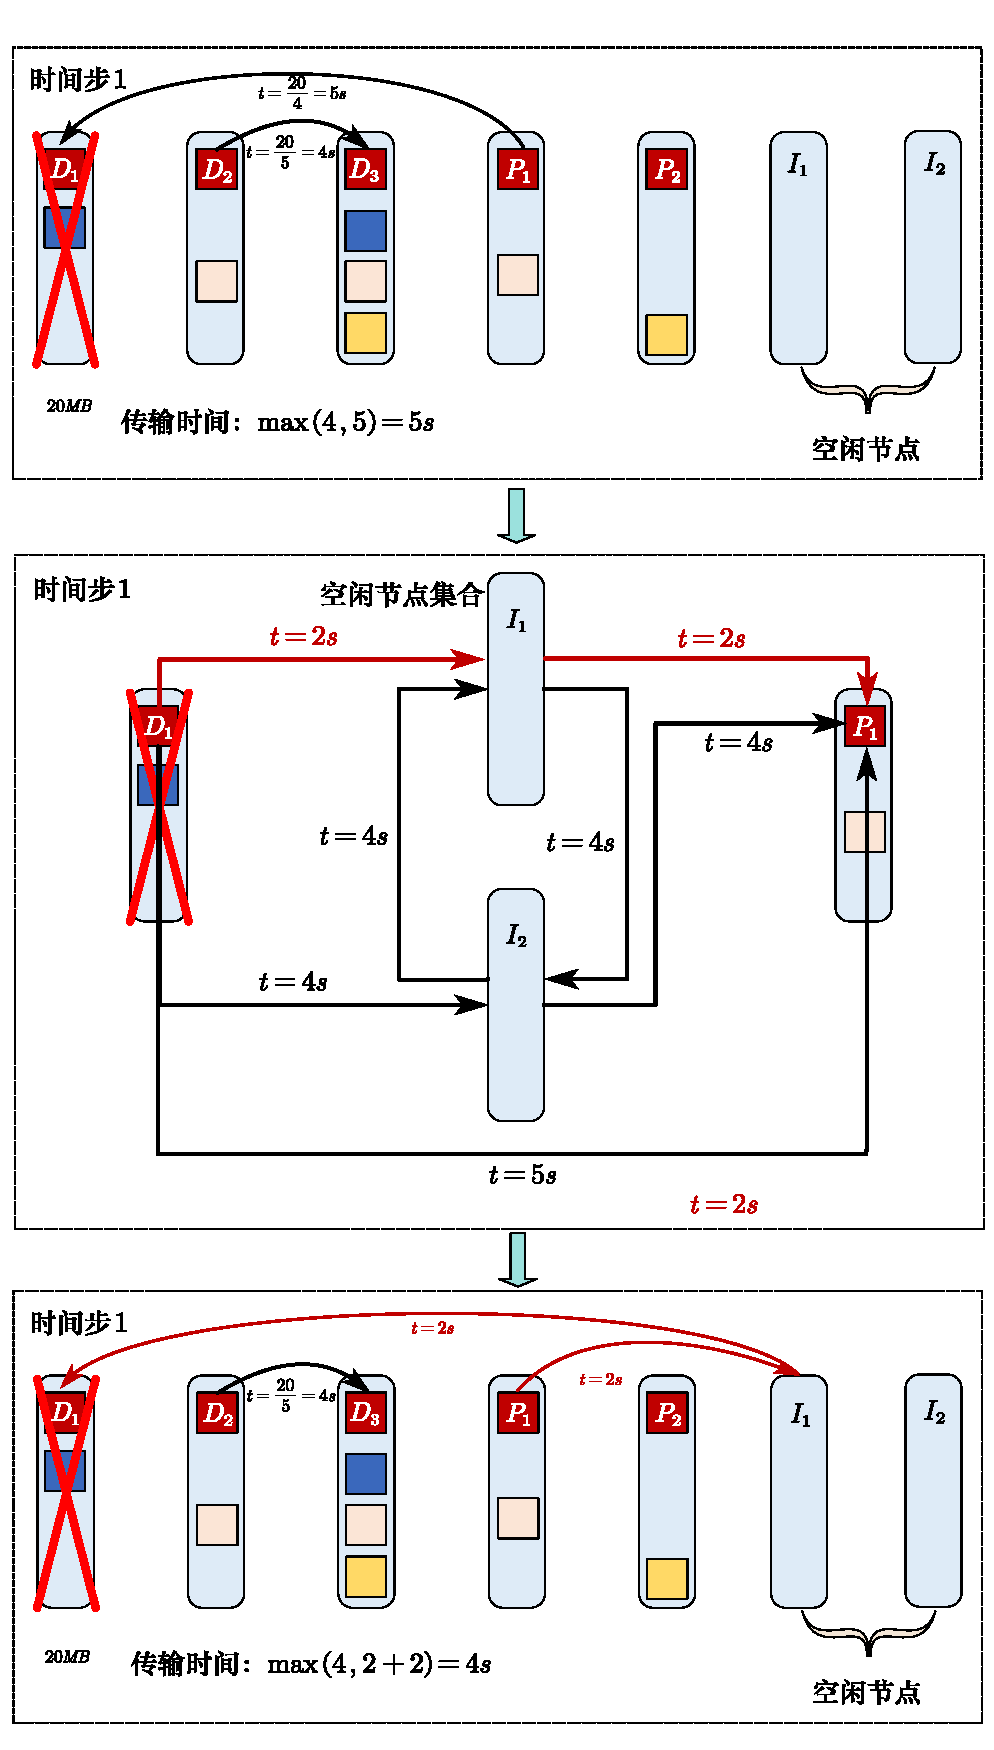
\includegraphics [scale=0.5]{figures/3.5.pdf}
	\caption{结合空闲节点的链路传输优化过程图}
	\label{fig:3.5}
\end{figure}

\section{实验结果与分析}

